\documentclass[12pt,doctor]{thesis}
\usepackage[margin=1.0in,includefoot,bindingoffset=6mm]{geometry}
\usepackage{footnote}
\usepackage{amsmath}
\usepackage{amsthm,amsbsy}
\usepackage{physics}
\usepackage{graphicx}
%\usepackage{fancyhdr}
%\usepackage{setspace}
\usepackage{enumerate}
%\setlength{\headheight}{15pt}
\usepackage[T1]{fontenc} % important for having seachable underscores
\usepackage{bm}
\usepackage[sort&compress,numbers]{natbib}
\usepackage{color}
%\setlength{\parskip}{2.54mm}
\usepackage{booktabs}
\usepackage[pagetoc,toc,titletoc,title]{appendix}
\usepackage{tocloft}

% for specifying urls and links
\usepackage{url}
\urlstyle{same} % same style as regular text

% citation and reference formatting
%\usepackage{apacite} % apa style citations, also change bibliographystyle below
\usepackage{cite} % math and engineering style citations

% define custom commands for creating references
% for tables, figures, equations and such
\newcommand{\eref}[1]{\eqref{#1}}        % cite equation
\newcommand{\fref}[1]{Figure~\ref{#1}}   % cite figure
\newcommand{\cref}[1]{Chapter~\ref{#1}}  % cite chapter
\newcommand{\sref}[1]{Section~\ref{#1}}  % cite section/sub(sub)section
\newcommand{\aref}[1]{Appendix~\ref{#1}} % cite appendix
\newcommand{\tref}[1]{Table~\ref{#1}}    % cite table

% Print only chapters in the Table Of Contents
\setcounter{secnumdepth}{2}
\setcounter{tocdepth}{2}

% Ensure that blank pages don't have numbers or heading on them
\makeatletter
\def\cleardoublepage{\clearpage\if@twoside \ifodd\c@page\else
 \hbox{}
 \vspace*{\fill}
 \thispagestyle{empty}
 \newpage\fi\fi}
\makeatother

%\pagestyle{plain}

\newcommand{\Red}[1]{\textcolor{red}{#1}}
\newcommand{\Blue}[1]{\textcolor{blue}{#1}}

% reset vec and hat style to a bold type
\let\oldhat\hat
\renewcommand{\hat}[1]{\oldhat{\mathbf{#1}}}
\renewcommand{\vec}[1]{\mathbf{#1}}
% stretches the vertical spacing of arrays/matrices
\renewcommand{\arraystretch}{2}
\setlength{\jot}{10pt}

\newcommand{\ham}{\mathcal{H}}
\newcommand{\MN}{\mathcal{M}}
\newcommand{\ke}{k_{\epsilon}}
\newcommand{\kpm}{k_{\pm}}
\newcommand{\sx}{\sigma_x}
\newcommand{\sy}{\sigma_y}
\newcommand{\sz}{\sigma_z}
\newcommand{\so}{\sigma_0}
\newcommand{\cc}{c^{\dagger}}
\newcommand{\de}{\Delta}

\graphicspath{ {./figures/} }
\title{Emergent Topological Phenomena in Low-D Systems Induced by Gauge Potentials}
\author{Aidan Winblad}
% department name
\email{acwinblad@gmail.com}
\department{Department of Physics}

% semester of completion
\semester{Fall 2023}

% committee member names
\advisor{Hua Chen}
\committee{Richard Eykholt}
\committee{Martin Gelfand}
\committee{Olivier Pinaud}

\mycopyright{%
Copyright by Aidan Winblad 2023 \\
All Rights Reserved
}

\abstract{Abstract goes here}

\acknowledgements{%
I would like to thank the CSU Graduate Student Council and the CSU Graduate School for initiating, commissioning and supporting this project.  I would also like to thank Nicole Ramo for her support and ensuring that we followed through with this project to completion.  I would like to thank Leif Anderson, who created and supported the previous LaTeX template for a number of years.  Although I have never met Leif, his work was invaluable in the creation of this package and has helped many students get their thesis approved by the CSU graduate school.  Finally, I would like to thank everyone who helps to contribute to this package.  Your work will help many CSU graduate students to create professional, beautiful and compelling theses and dissertations using LaTex.  Last but not least, thank you to the creators and maintaners of \LaTeX{} for creating a fantastic typesetting tool.
}

\begin{document}
\frontmatter

\maketitle              % insert title page
\makemycopyright        % insert copyright page
\makeabstract           % insert abstract page
\makeacknowledgements   % insert acknowledgements page

% any extra preliminary pages can be added here
% below is an example of a dedication page
% the dedication page is optional
\prelimtocentry{Dedication} % add table of contents entry
\begin{flatcenter} % center without extra space

    % page title
    DEDICATION

    %\vspace{3em} % place at top
    \vfill % or center on page

    \noindent \textit{I would like to dedicate this dissertation to my dog Zeta.}
    \vfill % fill extra space at bottom
\end{flatcenter}
\newpage

\tableofcontents    % insert table of contents
\listoftables       % insert list of tables (optional)
\listoffigures      % insert list of figures (optional)

\mainmatter % starts thesis body


\chapter{Introduction}
\Blue{EM gauge potential appears in electronic Hamiltonian in CM}
\begin{enumerate}
  \item \Blue{Review Maxwell theory -> gauge potential}
  \item \Blue{Minimal coupling $-i \hbar \nabla \rightarrow -i \hbar \nabla + q \vec{A}$ or $-i\partial_{\mu} \rightarrow -i\partial_{\mu} + qA_{\mu}$}
  \item \Blue{TB Hamiltonian and Peierls phase}
\end{enumerate}

\Blue{Topological phenomena in CM considered in thesis}
\begin{enumerate}
  \item \Blue{(1) Majorana and TSC}
  \begin{enumerate}[i]
    \item \Blue{Kitaev chain (\MN --- topological invariant). BdG?}
    \item \Blue{Braiding (Application in TQC)}
  \end{enumerate}
  \item \Blue{Landau Level and Hofstadter butterfly}
  \begin{enumerate}[i]
    \item \Blue{solve for LL in 2DEG --- why it's topological, chern number, TKNN quantum Hall}
    \item \Blue{square lattice --- hofstadter butterfly ( on other lattices, honeycomb)}
  \end{enumerate}
\end{enumerate}

STUFF
\chapter{Superconducting Triangular Islands as a Platform for Manipulating Majorana Zero Modes}

\begin{enumerate}
  \item \Blue{Introduction}
  \item \Blue{Formalism}
  \begin{enumerate}[i]
    \item \Blue{BdG --- decide how much detail on derivation}
    \item \Blue{Majorana Number}
    \item \Blue{Many-Body Berry Phase}
  \end{enumerate}
  \item \Blue{Model, results (uniform and non-uniform)}
  \item \Blue{Discussion, future}
\end{enumerate}

\section{Kitaev Triangle and Peierls substitution}

We start with a spinless or spin-polarized \textit{p}-wave superconductor

\begin{equation}
  \ham = \sum_{\langle j, l \rangle} (-t\cc_{j} c_l + \de e^{i\theta_{jl}} c_{j} c_l + h.c.) - \sum_j \mu \cc_j c_j,
\end{equation}
where $t$ is the hopping amplitude, $\de$  is the amplitude of (2D) \textit{p}-wave pairing, $\mu$ is the chemical potential, $\theta_{jl}$ is the polar angle of $\vec{r}_{jl} = \vec{r}_l - \vec{r}_j$, consistent with $\{\cc_l, \cc_j\} = 0$.

We will now include a gauge potential via a Peierls substitution as
\begin{align}\label{eq:HBdG}
  \cc_j &\rightarrow \cc_j \exp(-\dfrac{i e}{\hbar} \int_0^{\vec{r}_j} \vec{A} \cdot d\vec{l}), \nonumber \\
  \cc_j c_l &\rightarrow \cc_j c_l \exp(\dfrac{i e}{\hbar} \int_{\vec{r}_j}^{\vec{r}_l} \vec{A} \cdot d\vec{l}) \nonumber \\
  &\rightarrow \cc_l c_j e^{i \phi_{j,l}}. \nonumber \\
  \phi_{jl} &= \dfrac{e}{\hbar} \int_{\vec{r}_j}^{\vec{r}_l} \vec{A} \cdot d\vec{l} = -\phi_{lj}
\end{align}

The modified Hamiltonian is then
\begin{equation}
  \ham = \sum_{\langle j, l \rangle} (-t e^{i\phi_{jl}} \cc_{j} c_l + \de e^{i\theta_{jl}} c_{j} c_l + h.c.) - \sum_j \mu \cc_j c_j,
\end{equation}

The complex fermion operator can be written in the Majorana Fermion basis, a superposition of two Majorana fermions $c_j = \frac{1}{2} (a_j + i b_j)$.
Due to the nature of Majorana fermions, $a^{\dagger}_j = a_j$, the creation operator is $\cc_j = \frac{1}{2} (a_j - i b_j)$.
It is quickly seen after substitution we arrive at

\begin{align}
  \cc_j c_j &= \frac{1}{2} (1 + i a_j b_j), \\
  \cc_j c_l &= \frac{1}{4} (a_j a_l + b_j b_l + i a_j b_l - i b_j a_l), \\
  c_j c_l &= \frac{1}{4} (a_j a_l - b_j b_l + i a_j b_l + i b_j a_l).
\end{align}
The hopping term in MF basis are

\begin{equation}
  -t ( e^{i\phi_{jl}} \cc_j c_l + e^{-i\phi_{jl}} \cc_l c_j) = -\dfrac{it}{2} ( \sin\phi_{jl} (a_j a_l + b_j b_l) + \cos\phi_{jl} (a_j b_l - b_j a_l) ),
\end{equation}
the order parameter terms are

\begin{equation}
  \de ( e^{i\theta_{jl}} \cc_j \cc_l + e^{-i\theta_{jl}} c_j c_l) = \dfrac{i\de}{2} ( \sin\theta_{jl} (a_l a_j - b_l b_j) + \cos\theta_{jl} (a_l b_j + b_l a_j) ).
\end{equation}
Our Hamiltonian in MF basis is then

\begin{align}
  \ham =  - \dfrac{i}{2} \sum_{\langle j,l\rangle} [&(t\sin\phi_{jl}-\de\sin\theta_{jl}) a_j a_l + (t\sin\phi_{jl}+\de\sin\theta_{jl}) b_j b_l \nonumber \\
  +&(t\cos\phi_{jl}-\de\cos\theta_{jl}) a_j b_l - (t\cos\phi_{jl}+\de\cos\theta_{jl}) b_j a_l] \nonumber\\
  -\dfrac{i\mu}{2} \sum_j & a_j b_j
\end{align}

For concreteness we consider a 1-D chain in the Kitaev limit $t=\de$, $\mu=0$, and choose $phi_{jl}=0$ (either zero or a perpendicular gauge potential).
The Kitaev chain is resultant with $\ham = \sum_{j,j+1} -it b_j a_{j+1}$ and hosting MZM $a_1$ and $b_N$.


\section{Hollow Kitaev Triangles}
For systems with less fine-tuned Hamiltonians than the minimal model in the previous section, it is more instructive to search for MZM based on topological arguments.
In this section we show that MZM generally appear at the corners of a hollow triangle, which can be approximated by joining three finite-width chains or ribbons whose bulk topology is individually tuned by the same uniform vector potential.

To this end, we first show that topological phase transitions can be induced by a vector potential in a spinless $p$-wave superconductor ribbon.
In comparison with similar previous proposals that mostly focused on vector potentials or supercurrents flowing along the chain \cite{romitoManipulatingMajoranaFermions2012, takasanSupercurrentinducedTopologicalPhase2022}, we consider in particular the tunability by varying the direction of the vector potential relative to the length direction of the ribbon, which will become instrumental in a triangular structure.

Consider Eq.~\eqref{eq:HBdG} on a triangular lattice defined by unit-length lattice vectors $(\mathbf a_1, \mathbf a_2) = (\hat{x}, \frac{1}{2}\hat{x} + \frac{\sqrt{3}}{2}\hat{y})$ with $W$ unit cells along $\mathbf a_2$ but infinite unit cells along $\mathbf a_1$, and assume the Peierls phases are due to a uniform vector potential $\mathbf A$ so that $\phi_{jl} = \mathbf A\cdot \mathbf r_{jl}$.
We also introduce $\mathbf a_3 \equiv -\mathbf a_1 + \mathbf a_2$ for later convenience.
The Hamiltonian is periodic along $x$ and can be Fourier transformed through $\cc_{m,n} = \dfrac{1}{\sqrt{N}} \sum_{k} \cc_{k,n} e^{-i km}$, where $m,n$ label the lattice sites as $\mathbf r_{m,n} = m\mathbf a_1 + n \mathbf a_2$.
The resulting momentum space Hamiltonian can be written as the following block form up to a constant
\begin{eqnarray}\label{eq:Hribbon}
      \ham &=& \dfrac{1}{2} \sum_k \Psi_k^\dagger \left(
    \begin{matrix}
      h_t(k) & h_\Delta(k) \\
      h_\Delta^\dagger(k) & -h_t^*(-k)
    \end{matrix} \right)
    \Psi_k \\\nonumber
&\equiv&\dfrac{1}{2} \sum_k \Psi_k^\dagger H(k)
    \Psi_k
\end{eqnarray}
where $\Psi_k \equiv (c_{k,1},\dots, c_{k,W},c^\dag_{-k,1},\dots c_{-k,W}^\dag)^T$.
$h_t(k)$ is a $W\times W$ Hermitian tridiagonal matrix with $(h_t)_{n,n} = -2t\cos(k+\mathbf A\cdot \mathbf a_1) - \mu$ and $(h_t)_{n,n+1} = -t\left( e^{i(-k+\mathbf A\cdot \mathbf a_3)}  + e^{i\mathbf A \cdot \mathbf a_2}\right)$.
$h_\Delta(k)$ is a $W\times W$ tridiagonal matrix with $(h_\Delta)_{n,n} = -2i\de \sin k $ and $(h_\Delta)_{n,n\pm 1} = \mp \de\left[ e^{-i(\pm k + \frac{2\pi}{3})} + e^{-i\frac{\pi}{3}} \right]$.

By transforming Eq.~\eqref{eq:Hribbon} to the Majorana basis using the unitary transformation:
\begin{eqnarray}
    U\equiv \dfrac{1}{\sqrt{2}} \left(
  \begin{matrix}
    1 & 1 \\
    -i & i
  \end{matrix} \right) \otimes \mathbb{I}
\end{eqnarray}
where $\mathbb{I}$ is a ${W\times W}$ identity matrix, and defining $A_k\equiv -iU H(k) U^\dag$, not to be confused with the vector potential, one can calculate the Majorana number \cite{kitaevUnpairedMajoranaFermions2001} $\mathcal{M}$ of the 1D ribbon as \cite{liTopologicalSuperconductivityInduced2014}
\begin{eqnarray}
\mathcal{M} = {\rm sgn}\left[{{\rm Pf}(A_{k=0}) {\rm Pf}(A_{k=\pi})}\right]
\end{eqnarray}
where $\text{Pf}$ stands for the Pfaffian of a skew-symmetric matrix \cite{kitaevUnpairedMajoranaFermions2001}.
When $\mathcal{M} = -1$, the 1D system is in a nontrivial topological phase with MZM appearing at open ends of semi-infinite ribbons, and otherwise for $\mathcal{M} = 1$.

\begin{figure}[ht]
  \hspace{10pt}
  \subfloat[]{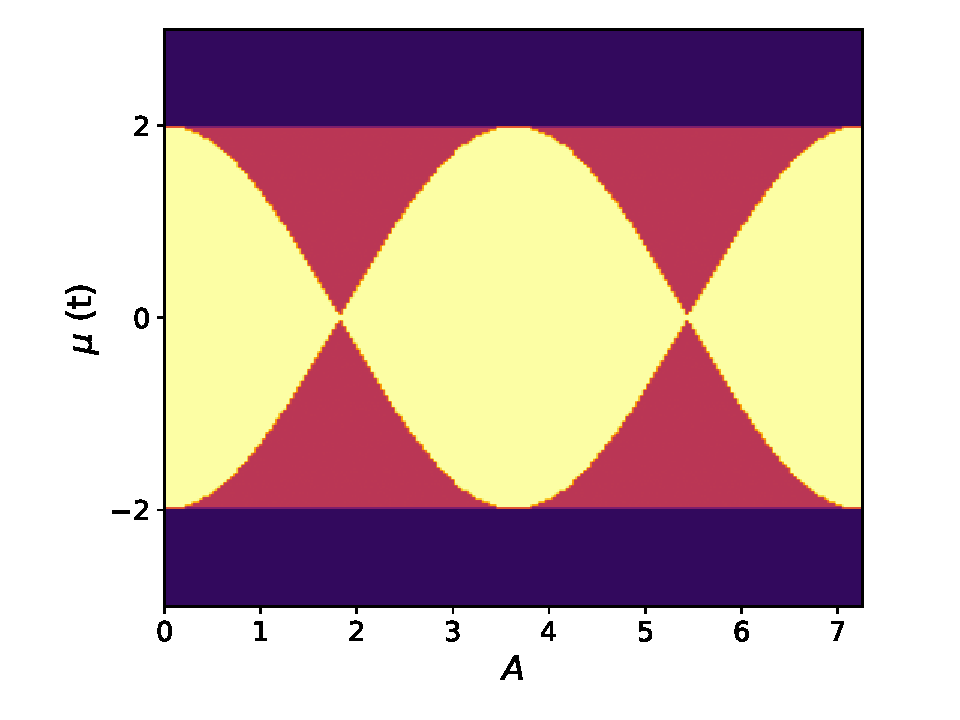
\includegraphics[width=0.53\textwidth]{topological-phase-diagram-1pi6-n-1.pdf}} \\
  \vspace{-15pt}
  \subfloat[]{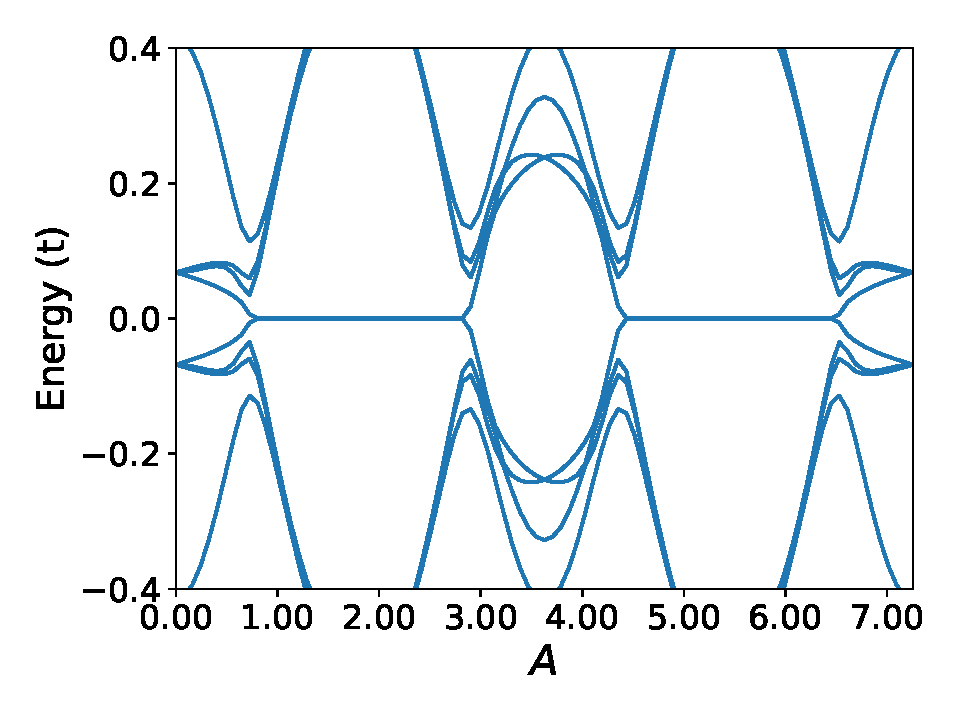
\includegraphics[width=0.50\textwidth]{spectral-flow-nr-50-w-1-mu-1_6.pdf}}
\caption{(a) Topological phase diagram for a $W=1$ triangular chain with the Hamiltonian Eq.~\eqref{eq:Hribbon} obtained by superimposing the $\mathcal{M}(A, \mu)$ plots of 1D chains with $\mathbf A = A\hat{y}$ and $\mathbf A = A(\frac{\sqrt{3}}{2}\hat{x}+\frac{1}{2}\hat{y})$. Color scheme: white---$\mathcal{M}=1$, dark blue---$\mathcal{M}=-1$, light blue---$\mathcal{M}=0$ (b) Near-gap BdG eigen-energies vs $A$ for a finite triangle with edge length $L = 50$, $W=1$, and $\mu=1.6$.}
  \label{fig: pd}
\end{figure}

In Fig.~\ref{fig: pd} (a) we show the topological phase diagrams for a 1D ribbon with width $W=1$, $\mathbf A = A\hat{y}$ and $\mathbf A = A(\frac{\sqrt{3}}{2}\hat{x}+\frac{1}{2}\hat{y})$ superimposed (see below).
We found that the vector potential component normal to the ribbon length direction has no effect on the Majorana number, nor does the sign of its component along the ribbon length direction.
However, topological phase transitions can be induced by varying the size of the vector potential component along the ribbon, consistent with previous results \cite{romitoManipulatingMajoranaFermions2012, takasanSupercurrentinducedTopologicalPhase2022}.
These properties motivate us to consider the structure of a hollow triangle formed by three finite-width ribbons subject to a uniform vector potential $\mathbf A = A\hat{y}$ as illustrated in Fig.~\ref{fig:triangles} (b).
The light blue color on the phase diagram Fig.~\ref{fig: pd} (a) therefore means that the bottom edge and the two upper edges of the hollow triangle have different $\mathcal{M}$, which should give rise to MZM localized at the two bottom corners if the triangle is large enough so that bulk-edge correspondence holds, and gap closing does not occur at other places along its edges.

To show that corner MZM indeed appear when the conditions given by the phase diagram Fig.~\ref{fig: pd} (a) are met, we directly diagonalize the BdG Hamiltonian of a finite hollow triangle with edge length $L=50$ and width $W=1$.
Fig.~\ref{fig: pd} (b) shows the spectral flow (BdG eigen-energies evolving with increasing vector potential $A$) close to zero energy at chemical potential $\mu=1.6$.
Indeed, zero-energy modes appear in the regions of $\mu$ and $A$ consistent with the phase diagram (except when the bulk band gap is too small; see \cite{supp} for some examples.).
Hollow triangles with larger larger $W$ also have qualitatively similar behavior, although the phase diagrams are more complex \cite{supp}.
The eigenfunctions for the zero-energy modes at $A=2.75$ and $\mu=1.6$ in Fig.~\ref{fig: rotation} (b) also confirm their spatial localization at the bottom corners of the triangle.

\begin{figure*}[ht]
  \hspace{-45pt}
  \subfloat[]{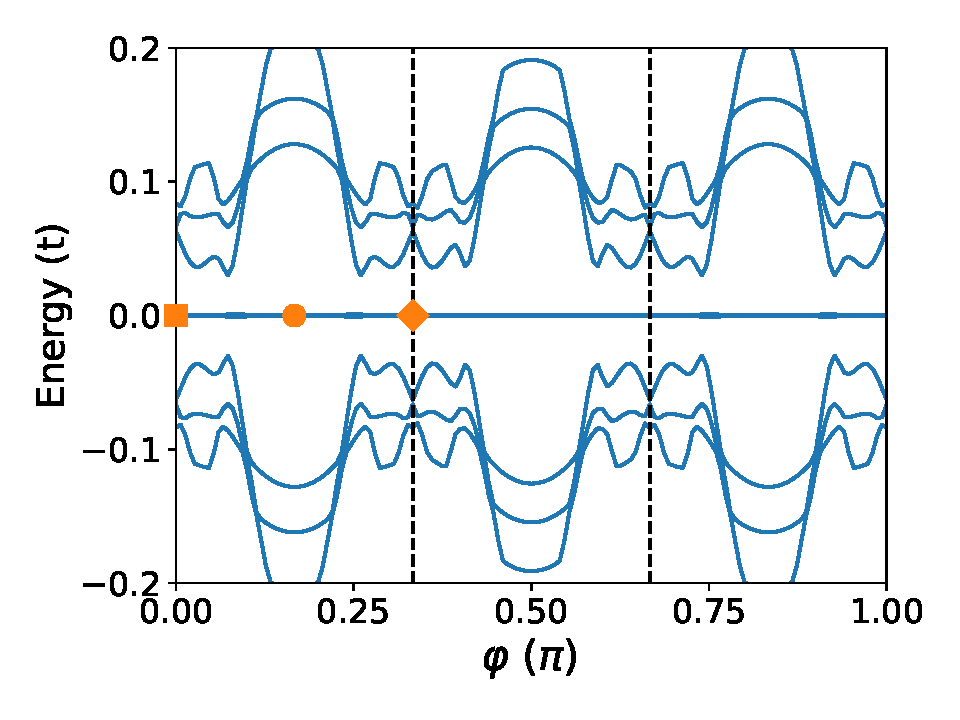
\includegraphics[height=150pt]{spectral-flow-rotation-constant-vector-nr-50-w-1-mu-1_6.pdf}} \\
  \subfloat[]{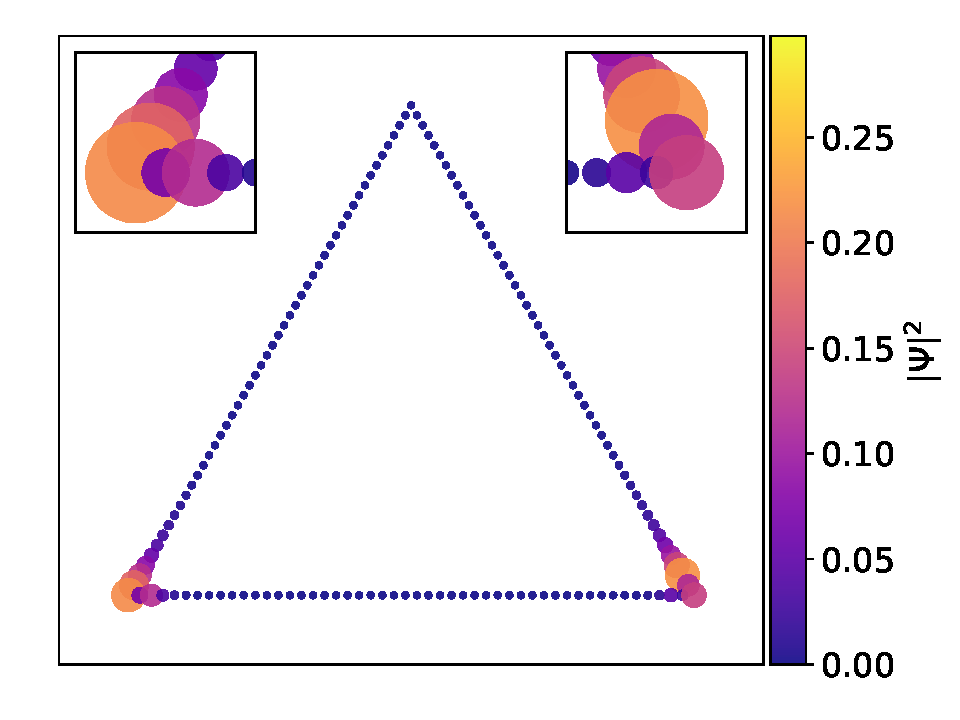
\includegraphics[height=125pt]{GS-T-Square.pdf}}\hspace{-20pt}
  \subfloat[]{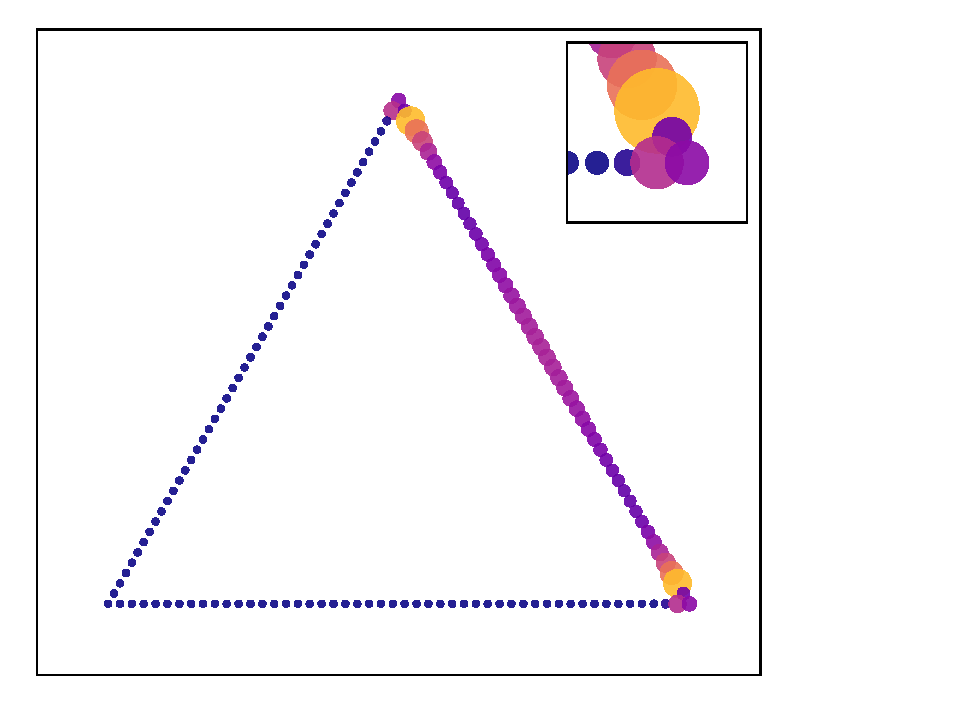
\includegraphics[height=125pt]{GS-T-Circle.pdf}}\hspace{-20pt}
  \subfloat[]{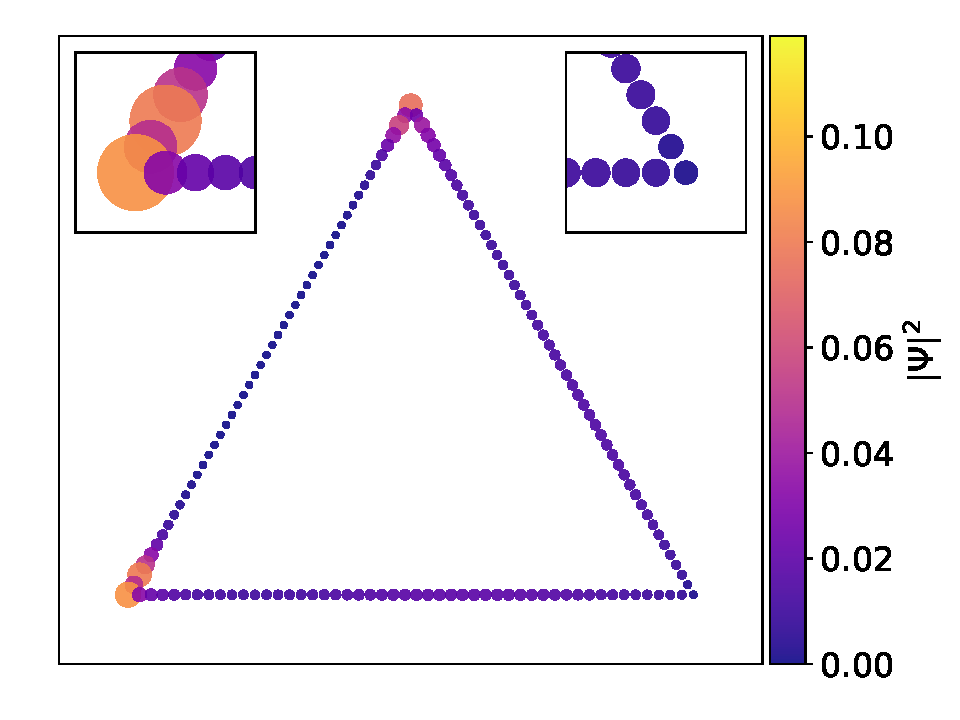
\includegraphics[height=127.5pt]{GS-T-Diamond.pdf}}
  \caption{(a) Spectral flow of a hollow triangle with $W=1$, $L=50$, $\mu=1.6$, and $A=2.75$ with increasing rotation angle $\varphi$, defined through $\mathbf A = A(-\sin\varphi \hat{x} + \cos\varphi \hat{y})$. (b-d) BdG eigenfunction $|\Psi|^2$ summed over the two zero modes at $\varphi = 0, \frac{\pi}{6}$, and $\frac{\pi}{3}$, respectively.}
  \label{fig: rotation}
\end{figure*}

We finally show that rotating the uniform vector potential in-plane can manipulate the positions of the MZM without hybridizing them with bulk states for certain ranges of $\mu$ and $A$.
Fig.~\ref{fig: rotation} (a) plots the spectral flow versus the in-plane azimuthal angle of $\mathbf A$, which clearly shows that the zero-energy modes persist throughout the rotation and the bulk gap never closes.
Figs.~\ref{fig: rotation} (b-d) plot the BdG wavefunctions of the MZM at special values of $\varphi$.
One can see that the two MZM appear to cycle through the three vertices by following the rotation of $\mathbf A$.
The robustness of the MZM therefore requires the condition of two edges being in a different topological phase from the third one to be satisfied throughout the rotation.
Such a criterion combined with the individual phase diagrams of the edges can help isolate the desired parameter regions of $\mu$ and $A$.
We also note that the positions of the MZM do not interchange after $\varphi$ increases from 0 to $\pi$, different from the situation of the minimal Kitaev triangle in Fig.~\ref{fig:3eig}.
The reason is that the MZM in the latter case are not due to bulk-boundary correspondence [the values of $A = \frac{2\pi}{3\sqrt{3}}$ and $\mu=0$ are a critical point in the phase diagram Fig.~\ref{fig: pd} (a)].
While the positions of the MZM at special points along the parameter path in the hollow triangle case have to be additionally constrained by the bulk topological phases of the three edges, that for the Kitaev triangle have more flexibility and are also protected by the finite size of the system.



\chapter{Floquet Landau Levels}

\begin{enumerate}
  \item \Blue{Introduction (Tahir's intro is fine, maybe in my own words, Floquet engineering)}
  \begin{enumerate}[i]
    \item \Blue{Time dependent, motivation---QAHE gap but not QHE gap}
    \item \Blue{Floquet Theorem--- quasi-energy spectrum}
  \end{enumerate}
  \item \Blue{Results}
  \begin{enumerate}[i]
    \item \Blue{square + \vec{A}(t) (Tahir's perturbative calc)}
    \item \Blue{honeycomb + \vec{A}(t) (Tahir's perturbative calc)}
  \end{enumerate}
  \item \Blue{Discussion and future}
\end{enumerate}

\chapter{Conclusion and Discussion}

\Blue{What makes gauge potential unique in creating/tuning/manipulating new topoglical systems}
\Blue{Applications}

\begin{appendices}
\chapter{Suitable Name}
\begin{enumerate}
  \item \Blue{Majorana Number derivation}
  \item \Blue{Other derivations not included in introduction}
\end{enumerate}
\end{appendices}

\end{document}

